%---A LaTeX template for Mechatronics ME 495 Capstone report.
\documentclass[twocolumn]{article}
\oddsidemargin=-0.35in
\topmargin=-0.75in
\headsep=0.1667in
\columnsep=0.25in
\textwidth=7.25in
\textheight=9.125in
\headheight=12pt

\usepackage{myfontstyle}			% Palatino & Euler fonts
\usepackage{graphicx}               % begin standard LaTeX macros
\usepackage{fancyhdr}               % fancy headers, see fancyhdr.pdf
\usepackage{fancyvrb}               % fancy verbatim environment, see fancyvrb.pdf
\usepackage{lastpage}               % used in the footer to specify the last page
\usepackage{amsmath}                % for log-like symbols
\usepackage{color}
\usepackage{dtklogos}
\newcommand{\bra}[1]{\langle #1|}
\newcommand{\ket}[1]{|#1\rangle}
\newcommand{\braket}[2]{\langle #1|#2\rangle} 

\begin{document}	%  <--- Here is where the document starts

\title{
	\vspace{-0.5in}\rule{\textwidth}{1pt}
	\begin{tabular}{ll}\begin{minipage}{4.75in}\vspace{6px}
			\noindent\Large Department of Mechanical Engineering\\
			\vspace{-12px}\\
			\noindent\large University of Washington\qquad 
		\end{minipage}&\begin{minipage}{2in}\vspace{6px}\small
		Stevens Way, Box 352600\\
		Seattle, WA 98195 USA\\
		206-543-5090
	\end{minipage}\end{tabular}
	\rule{\textwidth}{1pt}\vspace{0.25in}
	\Large
	Mechanical Impedance Control
}

\date{Mechatronics Capstone Design Report --- June 10, 2016}

\author{
	{Richard S Chen}\\
	rchen3@uw.edu
	\and 
	{Nathan Robert Dabling}\\
	ndabling@uw.edu
	\and
	{Fangzhong Guo}\\
	fzguo@uw.edu
	\and
	{James Kurniawan}\\
	kurnij@uw.edu
	\and
	{Kyle R Spangenberg}\\
	spangkyl@uw.edu
}

\maketitle



%---Executive Summary
\subsection*{Executive Summary{{\color{red}\ *}}}

Here is a suggested outline for Mechatronics ME 495 reports. Since the projects of all groups are different, feel free to modify the organization of this format to meet your project requirements. However, note that some sections ({\color{red}\bf{*}}) are required. 

%---Introduction
\subsection*{Introduction}

\noindent --Problem definition.

\noindent --Functional requirements

\noindent --Design approach, etc.

%---The Design
\subsection*{The Design}

\subsubsection*{ ---Description}

\subsubsection*{ ---Analysis}
Results of the modeling, MATLAB analysis, or other analysis that support the design.
\subsubsection*{ --- Mechanical}
\subsubsection*{ --- Electrical}
\subsubsection*{ --- Computational}
\subsubsection*{ --- Hardware}
\subsubsection*{ --- Software}
\subsubsection*{ --- Integration}   

%---Prototype
\subsection*{Prototype}
\subsubsection*{ --- Purpose}
\subsubsection*{ --- Description \& Implementation}
\subsubsection*{ --- Testing Results}Comparisons of experimental performance with the design analysis.

%---Risk and Liability

\subsection*{Risk and Liability{{\color{red}\ *}}}
The prototype for this project and its implicated future applications carry inherent risk due to the human interaction with moving parts and machinery. While the ultimate goal of this research is to enhance the interaction between humans and machines, one or both of them may fail during operation.

Specifically for the lab prototype there are certain fail-safes implemented to prevent injury. While not as large scale as some potential industrial and commercial applications, there is still risk to the user. The track, with the motor moving the belt and cart at potentially high velocities presents a pinching or collision hazard. Although the user's hand shouldn't be near the belt during operation, should such an event occur there is a switch box with an emergency stop button connected to the amplifier that can be pressed and will cut all power to the motor immediately. Through the switch box there also runs a set of limit switches that sit at the ends of the track. These prevent the cart from running off the end of the track or into the motor. If the user inputs a force that exceeds the limits of the system, a beeping noise will be triggered through the myRIO as a warning to lower or completely remove the input. Once the force input is back in the allowable range the beeping stops and the program is ready to continue.

The future industrial and commercial uses for this type of impedance control have more risk than the prototype. Implementation in a warehouse or factory will undoubtedly introduce more axes of motion. The use of more axes requires the user to be more aware of their surroundings as items are moved around. Care must also be taken when inputting parameters to ensure correct values are being used. Incorrect values may cause the system to not work and cause damage to the machine or human. If the system fails while lifting a heavy mass, the user will be unable to move or stop the mass, potentially endangering the user, bystanders, or the environment.

%---Ethical Issues
\subsection*{Ethical Issues{{\color{red}\ *}}}
asdflkasdfasdf
%---Impact on Society
%---Impact on Society
%Help Aging population get back to work, safe working conditions, rehabilitation
\subsection*{Impact on Society} \par
Impedance control systems are utilized in many different forms all around the world to improve people's lives, from helping senior citizens getting back into the workforce to physical rehabilitation.\par
In countries such as Japan and Singapore, where the aging population are straining the country's workforce, people have been looking into technologies which can help the senior citizens go back to work again. To do that, they came up with solutions which implemented impedance control methods such as motor-assisted pallet trucks and motor-assisted exosuits so as to help the seniors push and carry heavier loads and be on par with their younger counterparts. Moreover, these solutions can also be used by their younger counterparts to reduce strain on their body and create a safer working condition for everyone.\par
For many who had suffered injury to their arm, stroke, or spinal cord, they need to undergo rehabilitation treatment in order to regain full function and control of their arm again. By using a robot with a position-based impedance controller, the therapist will be able to ask the robot to assist or resist movement of the user's wrist, elbow, or shoulder in order to simulate arm movement conditions in daily life \cite{IEEE2006}.

%---Impact on the Environment
\subsection*{Impact on the Environment{{\color{red}\ *}}}

%---Cost and Engineering Economics
\subsection*{Cost and Engineering Economics{{\color{red}\ *}}}

%---Codes and Standards
\subsection*{Codes and Standards{{\color{red}\ *}}}

%---Conclusions
\subsection*{Conclusions{\color{red}\ *}}
\subsubsection*{ --- Continued Development}
\subsubsection*{ --- Final Product Configuration}

%---Bibliography
\subsection*{Bibliography{\color{red}\ *}}
-- Books, Articles, Data Sheets, etc., Cited in the body. 

See the \verb|.tex| file for the commands that build the following bibliography using \BibTeX. Examples of applications that can be used to manage the \BibTeX\  file include \verb|JabRef| (windows) and \verb|BibDesk| (os x).
\bibliographystyle{plain}		% (uses file "plain.bst")
\bibliography{Mechatronics}	% expects file "Mechatronics.bib"

%---Appendices
\subsection*{Appendices{\color{red}\ *}}
\subsubsection*{ --- Drawings}
\begin{enumerate}
\item{Mechanical}
\item{Electrical (individual components and connections)}
\item{Computer Hardware}
\item{Software Descriptions (flow charts, hierarchical diagrams, etc.)}
\end{enumerate}

\subsubsection*{ --- Code}
\begin{enumerate}
\item{MATLAB analysis and design}   {\color{red}\bf{*}}
\item{C-Code} {\color{red}\bf{*}}
\end{enumerate}
\subsubsection*{ --- Major components list for prototype}
\begin{enumerate}
\item{Manufacturer}
\item{Model number}
\item{Cost}
\end{enumerate}

\newpage
\subsubsection*{Here are some \LaTeX\ examples.} 

Examine the \verb|.tex| file to see how these were implemented.

\vspace{.167in}
A figure, with a graphic inserted from a \verb|.pdf| file, with a reference to the figure in the text.
\begin{figure}[htbp]
\begin{center}
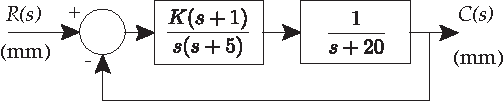
\includegraphics[width=2.75in]{ControlLoop2.pdf}
\caption{Control loop diagram}
\label{ControlLoop}
\end{center}
\end{figure}

Later on in the text: \dots We cite Figure \ref{ControlLoop} above.  Note the use of the \verb|\label{}| and \verb|\ref{}|.

Here are some numbered equations, with a reference.
\begin{equation}
T(s)=\frac{C(s)}{R(s)}=\frac{G(s)}{1+G(s)H(s)}
\label{eTF}
\end{equation}
\begin{equation}
\ket{f(x)} = \frac{1}{\sqrt{r}}\sum_{\ell=0}^{r-1}e^{2\pi i \ell/r}\ket{\hat{f}(\ell)}
\label{eFT}
\end{equation}

Elsewhere in  the text the equations \ref{eTF} and \ref{eFT} are cited. Note the use of the \verb|\label{}| and \verb|\ref{}|.

\vspace{.167in}
Here is an inline equation $f(t)=m\dot{v}(t)$. 
 
\vspace{.167in}
Some citations \cite{Bendat1971}, \cite{PhysRev.104.563}, \cite{Oppenheim1975}, and \cite{Papoulis1965}. 
 
\vspace{.167in}
A good \LaTeX\ reference is \cite{Lamport1994}.  See References.

\vspace{.167in}
The \verb|tabular| environment is tricky. 

But, it produces nice tables!

\vspace{.167in}
\begin{tabular}{|r||r@{--}l|p{1.25in}|}
\hline
\multicolumn{4}{|c|}{GG\&A Hoofed Stock}  \\  \hline  \hline
&\multicolumn{2}{c|}{Price}& \\ \cline{2-3}
\multicolumn{1}{|c||}{Year}
& \multicolumn{1}{r@{\,\vline\,}}{low}
& high & \multicolumn{1}{c|}{Comments} \\ \hline
1971 & 97 & 245 & Bad year. \\ \hline
72 & 245 &  245 & Light trading due to a heavy winter.  \\ \hline
73 & 245 & 2001 & No news was very good news this year. \\ \hline
\end{tabular}

\vspace{.5in}


\end{document}	%  <--- Here is where the document ends
